\documentclass[10pt]{beamer}

\usetheme{metropolis}

\usepackage{listings}
\usepackage{amssymb, amsmath}
\usepackage{tikz, tikz-cd}
\usepackage{adjustbox}
\usepackage{graphicx}

\newcommand{\hrsmall}{\noindent\makebox[\linewidth]{\rule{.3\paperwidth}{0.4pt}} \\}
\newcommand{\hr}{\noindent\makebox[\linewidth]{\rule{.7\paperwidth}{0.4pt}} \\}

\title{Differentiating Data Structures}
% \date{\today}
\date{}
\author{Mitch Stevens}
% \titlegraphic{\hfill\includegraphics[height=1.5cm]{logo.pdf}}

\begin{document}
 
\frame{\titlepage}

\begin{frame}[fragile] 
    \frametitle{What is an Algebra?}
    \begin{columns}[c] % the "c" option specifies center vertical alignment
    \column{.5\textwidth} % column designated by a command
	An \textbf{algebra} is a pair of monoids over some type. \\
    
    Examples of Algebras include: \\
    \begin{itemize}
        \item $\mathbb{B}$: (False, True, or, and)
        \item $\mathbb{N}, \mathbb{R}, \mathbb{C}$: ($ 0, 1, +, \times $)
        \item Sets: ($ \varnothing, U, \cup, \cap $)
        \item Polynomials of Algebras
        \item Square Matrices: ($ 0_n, I_n, +, \times $)
        \item Musical Notes: $\mathbb{Z}_{12}$
        \item Musical Sequences (Euterpea)
        \item Pretty Printing
        \item Image Composition
    \end{itemize}

    \column{.5\textwidth}
    \begin{lstlisting}[language=Haskell]
class Alg a where
  zero :: a
  one :: a
  (+) :: a -> a -> a
  (*) :: a -> a -> a
    \end{lstlisting} \\
    Laws: \\
    \begin{itemize}
        \item Monoid Laws
        \item $(a+b)*c = (a*c)+(a*c)$
    \end{itemize}

    \end{columns}
\end{frame}


\begin{frame}[fragile]
    \frametitle{Types form an Algebra}
    \begin{columns} % the "c" option specifiesdesignated by a command
    \column{.5\textwidth} % column maller types in two fundamental ways:
    A \textbf{sum type} takes a value from $A$ \textbf{or} from $B$
    \begin{itemize}
        \item \texttt{Either a b}
        \item \texttt{data Bool = True | False}
        \item \texttt{data Maybe a \\
    = Nothing | Just a}
    \end{itemize}
    \hrsmall
    A \textbf{product type} takes a value from $A$ \textbf{and} from $B$
    \begin{itemize}
        \item \texttt{(a, b)}
        \item \texttt{data Person = Person Name Age}
        \item \texttt{data Time = Time Hour Minutes Seconds}
    \end{itemize}

    \column{.5\textwidth}

    \begin{lstlisting}[language=Haskell]
instance Algebra Type where
  zero = Void
  one  = ()
  (+)  = Either
  (*)  = (,)
    \end{lstlisting}
    
    Does this satisfy the algebra law from earlier? \\
    $$(a+b)*c = a+c * b+c$$

    \end{columns}
\end{frame}
 

\begin{frame}[fragile]
    \frametitle{Type Isomorphism}
    \begin{columns} % the "c" option specifies center vertical alignment
    \column{.5\textwidth} % column designated by a command
    There is a difference between the set of Types and the equivalence class of types ($\mathbb{T}$)
    \hrsmall
    The size of a type is the number of values that can inhabit it. Lets call this size computing funtion
    $$ \sigma :: \mathbb{T} \rightarrow \mathbb{N} $$

    \column{.5\textwidth}
    \frame{
    \begin{tabular}{ ccc }
        Name & Constructor/Type & Size \\ 
        Void & N/A & 0 \\
        Unit & () & 1 \\
        Boolean & \texttt{False | True} & 2 \\
        Int & -2^{31} \hdots 2^{31} -1 & 2^{32} \\
        String & \texttt{[Char]} & \infty
    \end{tabular}
    }

    \end{columns}
\end{frame}


\begin{frame}[fragile]
    \frametitle{Calculating the size of a Type}
    \centering

    We can calculate $\sigma$ in a mechanical way using these rules:
    \begin{itemize}
        \item $\sigma(\text{Sum a b}) = \sigma(a) + \sigma(b)$
        \item $\sigma(\text{Prod a, b}) = \sigma(a) \times \sigma(b)$
        \item $\sigma(a \rightarrow b) \equiv \prod_{n=1}^{\sigma(a)} b  = \sigma(b)^{\sigma(a)}$
    \end{itemize}

    \hr

    \centering
    \begin{tabular}{ ccc }
        Name & Constructor/Type & Size \\
        Identity a & Identity a & \sigma(a) \\
        Maybe a & \texttt{Nothing | Just a} & 1 + \sigma(a) \\
        Either a b & \texttt{Left a | Right b} & \sigma(a) + \sigma(b) \\
        (a, b) & \texttt{Tuple a b} & \sigma(a) \times \sigma(b)
    \end{tabular}
    
\end{frame}


\begin{frame}[fragile]
    \frametitle{Traffic light example}
    \begin{columns} % the "c" option specifies center vertical alignment
    \column{.5\textwidth} % column designated by a command
    \begin{itemize}
        \item How many values inhabit \texttt{Traffic}?
        \item How many values inhabit \texttt{Intersection}?
        \item How many values inhabit \texttt{ComplexInter}?
    \end{itemize}

    \column{.5\textwidth}
    \begin{lstlisting}[language=Haskell]
data Traffic = R | Y | G

data Intersection = Inter
    { north :: Traffic
    , east  :: Traffic
    , south :: Traffic
    , west  :: Traffic
    }
        
type ComplexInter lane =
    lane -> Traffic
    \end{lstlisting}
    \end{columns}
\end{frame}


\begin{frame}[fragile]
    \frametitle{How many values inhabit List?}
    \begin{center}
        \begin{tabular}{ ccc }
            \sigma(\texttt{List a}) &=& \sigma(\texttt{Nil | Cons a (List a}) \\
                 &=& \sigma(\texttt{Nil}) + \sigma(\texttt{Cons a (List a)}) \\
                 &=& 1 + \sigma(a) \times \sigma(\texttt{List a}) \\
                 &=& 1 + a \times (1 + a \times \sigma(\texttt{List a})) \\
                 &=& 1 + a + a^2 \times \sigma(\texttt{List a}) \\
                 &=& 1 + a + a^2 \times ( 1 + a \times \sigma(\texttt{List a})) \\
                 &=& 1 + a + a^2 + a^3 + a^4 + \hdots
        \end{tabular}
    \end{center}
    \hr
    So we have:
    $$ \sigma(\texttt{List a}) = \sum_{n=0}^\infty a^n = \frac{1}{1 - a} $$\\
    Which strongly resembles the geometric sum ($\lvert r \rvert \ge 1$):
    $$ \sum_{n=0}^\infty r^n = \frac{1}{1 - r}$$

\end{frame}


\begin{frame}[fragile]
    \frametitle{Refactoring}
    Give that $\sigma$ is a isomorphism, we know that $id_\mathbb{T} = \sigma \circ id_\mathbb{N} \circ \sigma^{-1}$. \par
    
    \begin{center}
        \adjustbox{scale=1.5}{%
            \begin{tikzcd}[cramped]
                \mathbb{T} \arrow[r, "id_\mathbb{T}"] \arrow[d, "\sigma"]
                & \mathbb{T} \\
                \mathbb{N} \arrow [r, "id_\mathbb{N}"]
                & \mathbb{N} \arrow[u, "\sigma^{-1}"]
            \end {tikzcd}
        }
    \end{center}
    \hr
    Example: Refactoring the type $\texttt{Either (b, a, [b]) a}$
\end{frame}


\begin{frame}[fragile]
    \frametitle{One-Hole Contexts and Zippers}
    \centering
    A 'One-hole Context' is a data structure with a 'hole' where a value can be inserted. \\
    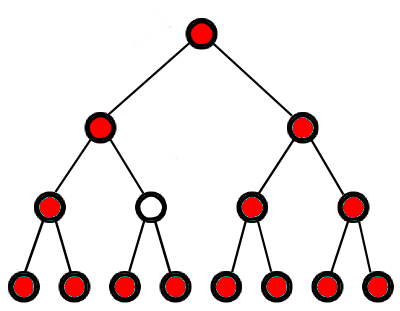
\includegraphics[height=100px]{one-hole_context.png} \\
    If you include a value, you can use a one-hole context to recreate the original data-structure. The product of a value and a one-hole context is called a zipper.
\end{frame}


\begin{frame}[fragile]
    \frametitle{Rules of Differentiation}
    \begin{columns} % the "c" option specifies center vertical alignment
    \column{.5\textwidth} % column designated by a command
    Usually only differentiation is only defined over functions $ \mathbb{R}^m \rightarrow \mathbb{R}^n $. But the rules that come from differential calculus can be applied to any algebra. \\
    This is not usually meaningful, however.
    

    \column{.5\textwidth}
    Sum Rule:
    $$ \partial_x (A+B) = \partial_x A \partial_x B $$ \\
    
    Product Rule:
    $$ \partial_x (A \times B) = \partial_x A \times B + A \times \partial_x B $$ \\

    Chain Rule:
    $$ \partial_x (A \circ B) = \partial_x A (B) \times \partial_x A $$

    \end{columns}
\end{frame}

\begin{frame}[fragile]
    \frametitle{Differentiating Types}
    The dervivative of a Type is meaningful, it is \textbf{exactly} the type of its one-hole context! \\

    It is easier to differentiate a function in $\mathbb{N}$ than a function in $\mathbb{T}$. We apply the same trick as before.

    \begin{center}
        \adjustbox{scale=1.5}{%
            \begin{tikzcd}
                \mathbb{T} \arrow[r, "\partial_\mathbb{T}"] \arrow[d, "\sigma"]
                & \mathbb{T} \\
                \mathbb{N} \arrow [r, "\partial_\mathbb{N}"]
                & \mathbb{N} \arrow[u, "\sigma^{-1}"]
            \end {tikzcd}
        }
    \end{center} \\

    

\end{frame}


\begin{frame}[fragile]
    \frametitle{The one-hole context of a List}
    
\end{frame}


\begin{frame}[fragile]
    \frametitle{Other Questions}
    \begin{itemize}
        \item Can we perform more than one differentiation? \\
            Yes.
        \item Is there a method for computing anti-differentiation? \\
            No idea.
        \item Is there a reasonable interpretation for a fractional or negative type? \\
            Kind of.
    \end{itemize} 

\end{frame}


\end{document}
    